\newpage
\section{Entwurf eines Task Scheduling Verfahrens}\label{sec:Gesamtkonzept}
Um die in Abschnitt \ref{sec:Datenerfassung} und \ref{sec:Datenverarbeitung} beschriebenen Teilsysteme zu einem lauffähigen Programm zusammenzuführen, wird ein Konzept benötigt, das es erlaubt, einzelne Aufgaben in regelmäßigen Intervallen auszuführen. Dieses Konzept kann durch die Verwendung eines TaskSchedulers realisiert werden, der die zeitliche Planung und Ausführung der einzelnen Aufgaben gemäß den festgelegten Intervallen steuern und verwalten kann. Hierzu werden unter dem \textit{HM.TimerBasedScheduler} Verzeichnis folgende Klassen angelegt. (Siehe Abbildung \ref{fig:TimerBasedScheduler}) 
\begin{center}
    \begin{figure}[h!]
        \centering
        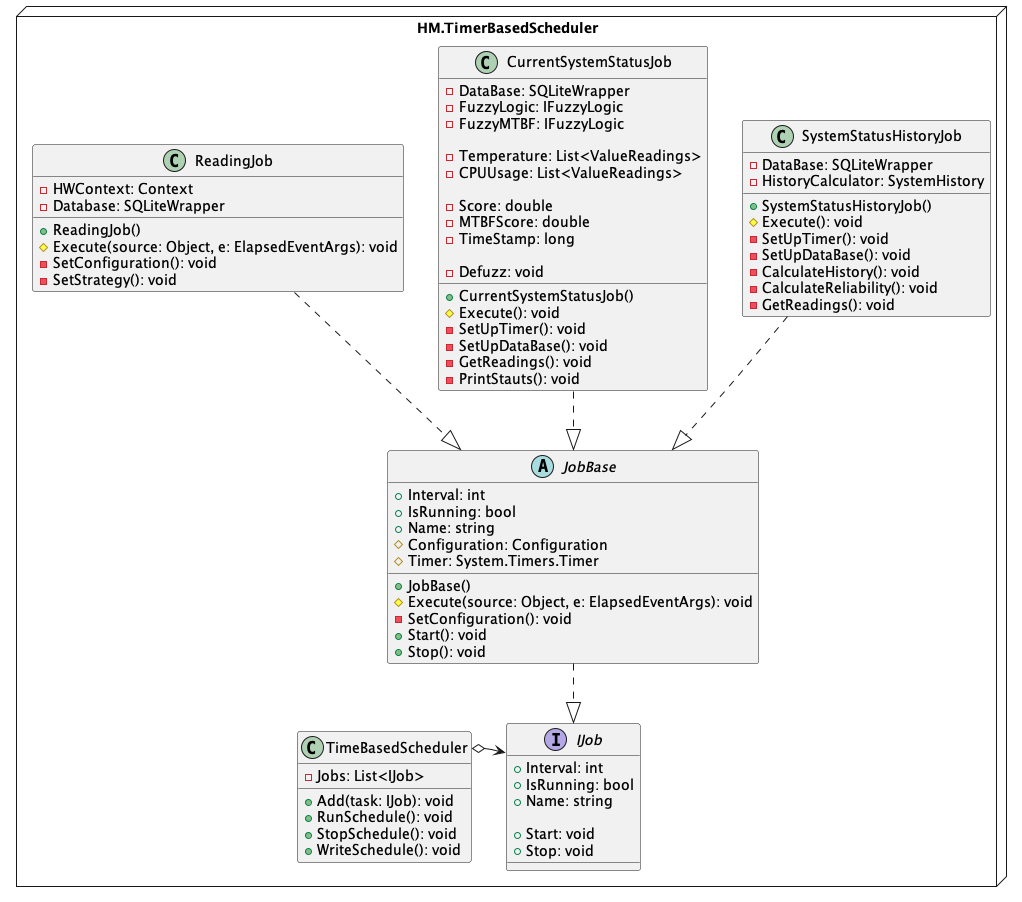
\includegraphics[width=1\textwidth]{HMTimerBasedScheduler.png}
        \caption{Architektur des Taskscheduler}
        \label{fig:TimerBasedScheduler}
    \end{figure}
\end{center}
Die Basis des Schedulers ist die \textit{TimerBasedScheduler} Klasse. In dieser können verschiedene Aufgaben zum Zeitplan hinzugefügt werden. Zudem kann der Scheduler in dieser Klasse gestartet und gestoppt werden. Um zur Laufzeit des Programms eine Übersicht über die laufenden Aufgaben zu haben, wird der \textit{TimerBasedScheduler} Klasse eine Funktion zur Visualisierung des Zeitplans in der Konsole hinzugefügt.\\
Die Schnittstelle zu einer bestimmten Aufgabe, im Weiteren als Job bezeichnet, wird über das \textit{IJob} Interface definiert. Dieses definiert die von der \textit{TimerBasedScheduler} Klasse verwendeten Funktionen und Variablen. Aus diesem wird anschließend die abstrakte \textit{JobBase} Klasse abgeleitet. Die \textit{JobBase} Klasse liefert alle Basisfunktionen und Variablen, welche in jedem Job verwendet werden. Die Verwendung einer Basisklasse verhindert Codeduplikation und erleichtert durch eine vordefinierte Struktur das Programmieren weiterer spezifischen Jobs.\\
Im letzten Schritt wird eine Reihe von Jobs abgeleitet, welche die in gewünschten Aufgaben ausführen. Hierzu werden drei Klassen aus der \textit{JobBase} Klasse abgeleitet.
\begin{itemize}
    \item \textbf{ReadingJob}\\
    Aufgabe der \textit{ReadingJob} Klasse ist die Auswertung der Hardwarespezifischen Sensoren. Hierzu bedient sich die Klasse dem in Abschnitt \ref{sec:AuslesenHardware} beschriebenen \textit{HM.HWServices} und dessen Strategieklassen. Zudem verwendete diese Klasse die, in Abschnitt \ref{sec:DatenbankModell} beschriebene, Datenbank Schnittstelle zum Schreiben der Messwerte. 
    \item \textbf{CurrentSystemStatusJob}\\
    Aufgabe der \textit{CurrentSystemStatusJob} Klasse ist die Ermittelung des aktuellen Systemstatus. Hierzu verwendet die Klasse das, in Abschnitt \ref{sec:SystemStatusErmittelung} beschriebene, \textit{HM.ScoringModel} Verzeichnis und dessen \textit{FuzzyLogic} Klassen. Des Weiteren bedient sich auch diese Klasse der in Abschnitt \ref{sec:DatenbankModell} beschriebene Datenbank Schnittstelle.
    \item \textbf{SystemStatusHistoryJob}\\
    Aufgabe der \textit{SystemStatusHistoryJob} Klasse ist die Ermittelung der Systemstatus Historie so wie der Systemzuverlässigkeit. Hierzu verwendet die Klasse das, in Abschnitt \ref{sec:SystemHistoryReliability} beschriebene \textit{HM.ScoringModel} Verzeichnis und dessen \textit{StatusHistory} Klasse. Des Weiteren bedient sich auch diese Klasse der in Abschnitt \ref{sec:DatenbankModell} beschriebene Datenbank Schnittstelle. Des Weiteren bedient sich auch diese Klasse der in Abschnitt \ref{sec:DatenbankModell} beschriebene Datenbank Schnittstelle.    
\end{itemize}
